\chapter{Предисловие}
Здравствуй, мой дорогой читатель. Написать данное учебное пособие было титаническим трудом. Но я думаю, что я и мои коллеги справились достойно.

Данное учебное пособие предназначено для подготовки конкретно к устному ГОСу по математике. Как вы уже поняли, оглавление представляет собой программу к ГОСУ 2016 года. Заметьте, что она <<кликабельна>>, так что умелые люди при должной сноровке смогут быстро на экзамене найти почти любой материал, который касается именно программы ГОСа. И <<кликабельно>> не только оглавление данной книги, но и всевозможные числа и названия, указывающие на теоремы, которые уже использовались ранее в книге. Надеюсь, это кому-нибудь поможет. 

Надо бы отметить для любителей учебников и лекций определенных авторов, что я писал билеты, существенно опираясь на учебные пособия, лекции различных преподавателей. Вот список соответствия билетов из программы и названий курсов от кафедры высшей математики материалам, которыми я в основном пользовался (подчеркиваю, в основном, ведь бывало я по хорошему предложению из каждой книги брал):
\begin{itemize}
\item[\textit{1-6}]
\; --- \: \textit{Введение в математический анализ.} 

Лекции Сакбаева В.Ж. и учебное пособие Яковлева Г.Н. (часть 1), учебное пособие Бесова О.В.
\item[\textit{7-8}] 
\; --- \: \textit{Многомерный анализ, интегралы и ряды.}

Лекции
\item[\textit{9-10}] 
\; --- \: \textit{Кратные интегралы и теория поля.}

Лекции
\item[\textit{11-13}] 
\; --- \: \textit{Многомерный анализ, интегралы и ряды.}

Лекции
\item[\textit{14-16}] 
\; --- \: \textit{Кратные интегралы и теория поля.}

Лекции
\item[\textit{17-19}] 
\; --- \: \textit{Гармонический анализ.}

Лекции Сакбаева В.Ж. и учебное пособие Яковлева Г.Н. (часть 3).
\item[\textit{20}] 
\; --- \: \textit{Аналитическая геометрия.}

Лекции Чубарова И.А. и учебное пособие Беклемишева Д.В.
\item[\textit{21-25}] 
\; --- \: \textit{Линейная алгебра.}

Лекции Чубарова И.А. и учебное пособие Беклемишева Д.В.
\item[\textit{26-29}] 
\; --- \: \textit{Дифференциальные уравнения.}

Лекции
\item[\textit{30-32}]
\; --- \: \textit{Теория вероятностей.}

Лекции Райгородского А.М., семинарские записи Карлова М.И., учебное пособие Гнеденко Б.В., учебное пособие трех авторов: Захарова В.К., Севастьянов Б.А., Чистякова В.П.
\item[\textit{33-36}]
\; --- \: \textit{Теория функций комплексного переменного.}

Лекции Карлова М.И. и учебное пособие Половинкина Е.С.
\end{itemize}

\mbox{}

\begin{wrapfigure}{r}{0.51\textwidth}
\vspace{-\baselineskip}
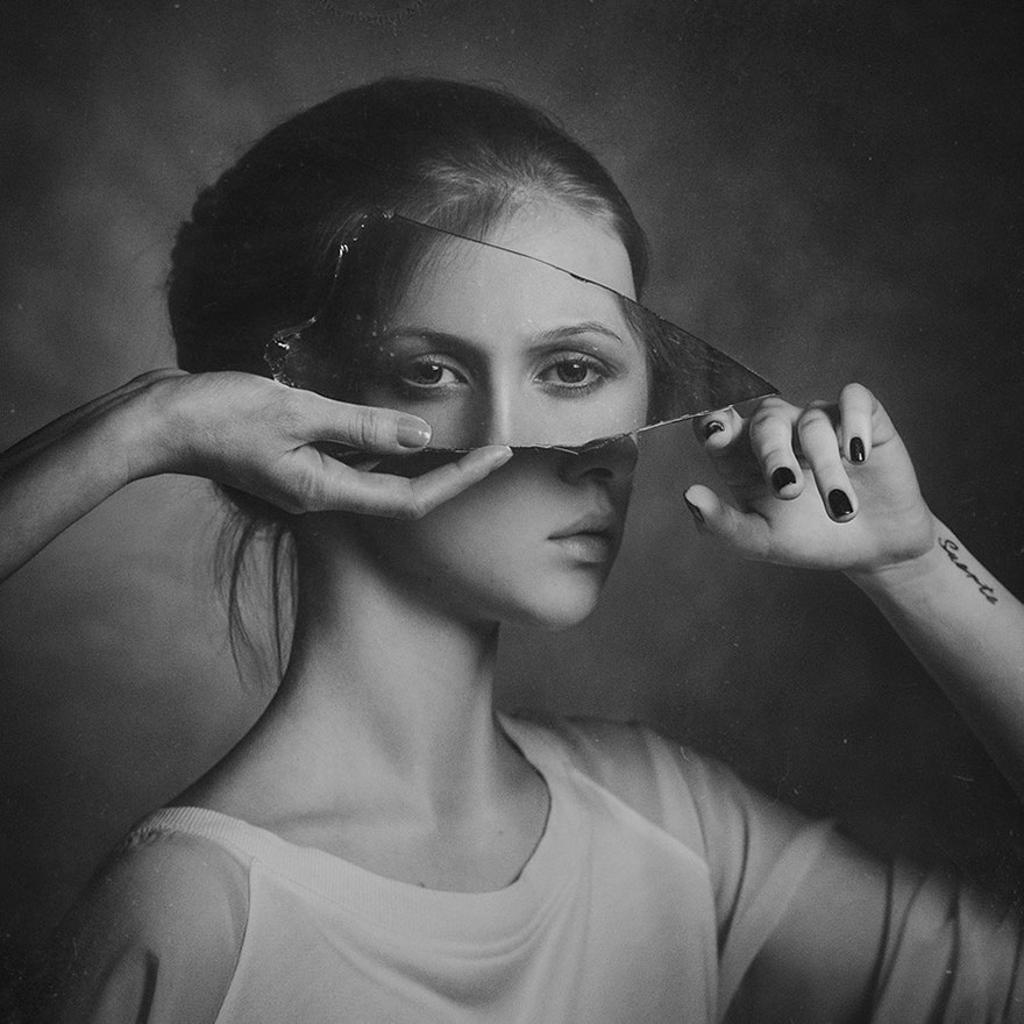
\includegraphics[width=0.51\textwidth]{pictures/love}
\end{wrapfigure}
Я был предельно внимателен к составлению данной книги, стараясь уменьшить количество опечаток и повысить качество излагаемого материала. Но я отказываюсь от ответственности за всевозможные недочеты в этой книге, ведь я, на данный момент, всего лишь студент 3-ого курса, а главное --- человек, который может ошибаться. И поэтому, прошу Вас не забывать отправить мне (ссылка ниже) сообщения о любых неточностях, опечатках, ошибках (даже о таких, как, например, <<забыл точку поставить>>). Также пишите, если хотите дать совет или выразить любые личные пожелания. 

Хочется выразить особую благодарность Артемию Лузянину, Проскину Роману и Кудашову Аркадию за соучастие в написании этой книги.
 
\vspace*{\baselineskip}
\hyphenation{ГОСе}

Желаю всем отличных результатов~на~ГОСе.

\mbox{}

\noindent Диденко А. 

\noindent\href{https://vk.com/didenko.andre}{$https://vk.com/didenko.andre$}

\mbox{}

\noindent PS. Мы можете сами помочь нам своими действиями, сделав Pull Request в следующем репозитории:

\noindent\href{https://github.com/DidenkoAndre/GOS_book}{$https://github.com/DidenkoAndre/GOS\_book$}